\subsubsection{Visitor scenarios}
\subsubsection*{Scenario 1}
Prabaker, a farmer from Telangana, wants to know how is the trend of agriculture in his country and for this reason he wants to have access to data about this. A friend of him, Sundar, suggested him to visit Dream’s web page, a project by the United Nations of India, giving him the link. Prabaker opens the link and connects to the site’s home page, where he can access different data set. Once he clicks on the button "Access the data" he notices that there’s the possibility to select different filters to see information coming from the various districts of Telangana. He decides to select the filter that shows how much rain has fallen in the last 24 hours in the zone of his land holding because in the monsoon season is important to keep track of it in order to not waste the crop. The page is rendered and he can see the updated data on screen.

\subsubsection*{Scenario 2}
Matteo, a researcher, needs to analyze soil quality data of the Telengana region about last month for his study in resource efficiency for crops in developing countries. He learns about project Dream that allows free access to all the resources he needs for his study. So Matteo connects to the Dream home page and then he selects the button to access the data. After doing that a new page is rendered and selecting a data set and scrolling down on it, he notices the possibility to download the data in different formats. He selects the one he suits the most and clicks on the button download.
\newpage

\subsubsection*{Use case diagram}
    \begin{figure}[hbt!]
        \centering
        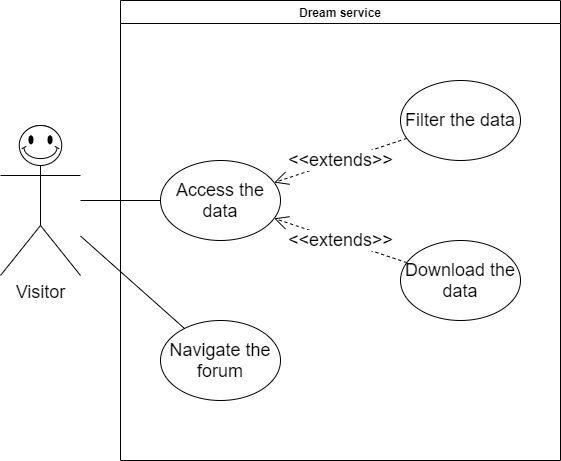
\includegraphics[scale=0.40]{images/use_cases_diagram/visitor_use_case.png}
        \caption{Use case diagram}
        \label{fig:vistor_use_case}
    \end{figure}
\FloatBarrier
    
\subsubsection*{Use case tables}

\begin{longtable}{p{.25\textwidth} | p{.75\textwidth}}
\caption{Filter data}
    \label{tab:filter_data}\\
        \hline
        \textbf{ID} & 1\\
        \hline
        \textbf{Name}  &  Filter data\\
        \hline
        \textbf{Actor}  &  Visitor\\
        \hline
        \textbf{Entry condition}  & The Visitor is in the Dream home page\\
    
        \hline
        \textbf{Events flow} & \begin{itemize}
                \item The Visitor clicks on the "Access the data" button
                \item The system displays the available data.
                \item The Visitor searches for the data set of interest
                \item The Visitor selects the “Filter” button on the data set he wants to filter
                \item The System pops up a list of different filters that can be applied to do a more precise search
                \item The Visitor select all the filters he wants to apply
                \item The Visitor clicks on the “Search” button
                \item The System search applying the selected filters

                \end{itemize}
                 \\
        \hline
        \textbf{Exit condition} & The new search is displayed\\
        \hline
    

    \end{longtable}
     \begin{figure}[h!]
        \centering
        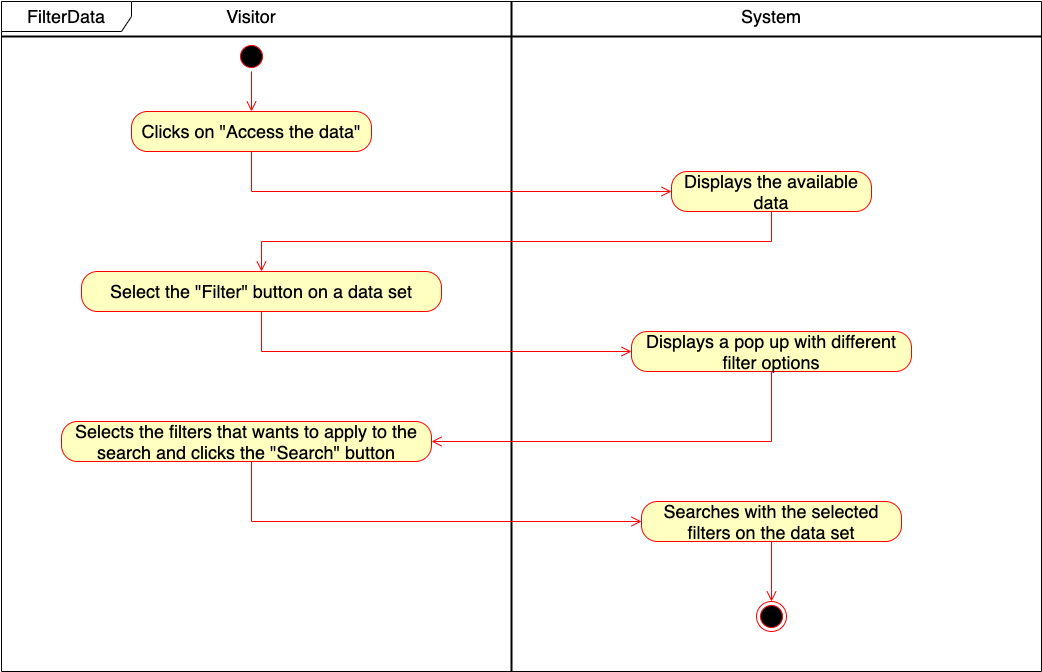
\includegraphics[scale=0.35]{images/use_cases_diagram/visitor_filter_data.png}
        \caption{Filter data}
        \label{fig:filter_data}
    \end{figure}
   
    \FloatBarrier
    \begin{longtable}{p{.25\textwidth} | p{.75\textwidth}}
    \caption{Download data set}
    \label{tab:download_dataset}\\
        \hline
        \textbf{ID} & 2\\
        \hline
        \textbf{Name}  &  Download data set\\
        \hline
        \textbf{Actor}  &  Visitor\\
        \hline
        \textbf{Entry condition}  &  The Visitor is in the Dream home page\\
        \hline
        \textbf{Events flow} & \begin{itemize}
                \item The Visitor clicks on the "Access the data" button
                \item The system displays the available data.
                \item The Visitor search for the data set of interest
                \item The Visitor select the “Download” button on the data set he wants to download
                \item The System pops up a data panoramic showing the different formats in which the data can be downloaded
                \item The Visitor select the data format he prefers
                \item The Visitor clicks on the “Download” button
                \item The System starts the download

                \end{itemize}
                 \\
        \hline
        \textbf{Exit condition} &  The data set is downloaded\\
        \hline
        \textbf{Output} & Data set\\
        \hline
    
    \end{longtable}
    \newpage
\begin{figure}[h!]
        \centering
        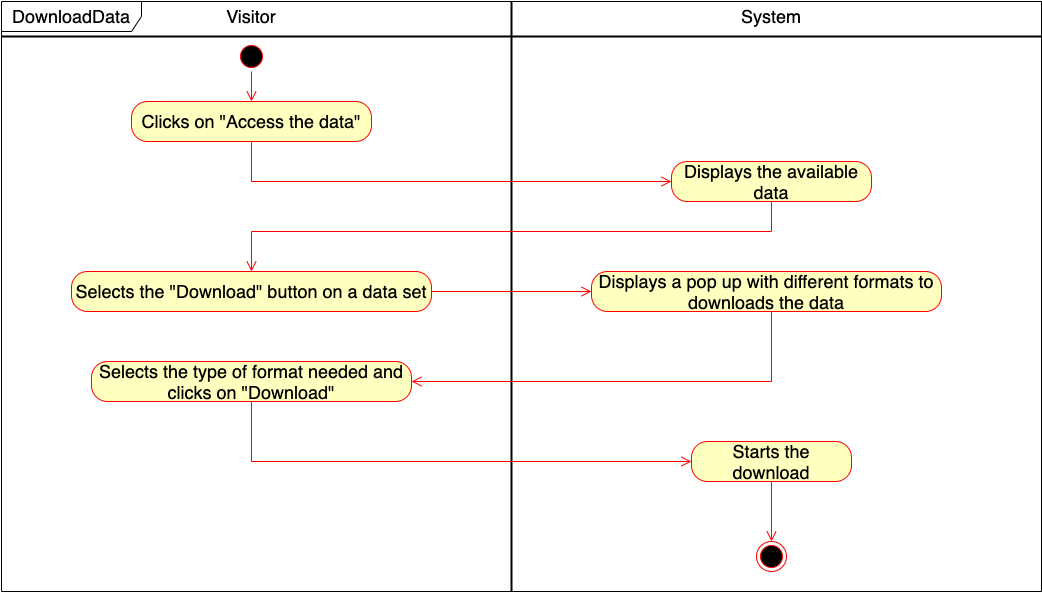
\includegraphics[scale=0.30]{images/use_cases_diagram/visitor_download_dataset.png}
        \caption{Download data set}
        \label{fig:download_data}
    \end{figure}
    \FloatBarrier
    
\begin{longtable}{p{.25\textwidth} | p{.75\textwidth}}
    \caption{Navigate the forum and download a document}
    \label{tab:navigate_forum}\\
        \hline
        \textbf{ID} & 3\\
        \hline
        \textbf{Name}  &  Navigate the forum and download a document\\
        \hline
        \textbf{Actor}  &  Visitor\\
        \hline
        \textbf{Entry condition}  &  The Visitor is in the Dream home page\\
        \hline
        \textbf{Events flow} & \begin{itemize}
                \item The Visitor click on "Open the forum" button
                \item The Visitor is redirected in the forum home page where all the topics are visible
                \item The Visitor click on the topic of his interest
                \item The System displays all the discussion related to the chosen topic
                \item The Visitor select the discussion he is interested in
                \item The system displays the discussion published by the Policy maker with all the replies from different users.
                \item The Visitor click and start the download of the attachment contained in the Policy maker's relation. 
                \end{itemize}
                 \\
        \hline
        \textbf{Exit condition} &  The visitor download the document\\
        \hline
        \textbf{Output} & Attachment \\ \hline
    
    \end{longtable}
\begin{figure}[h!]
        \centering
        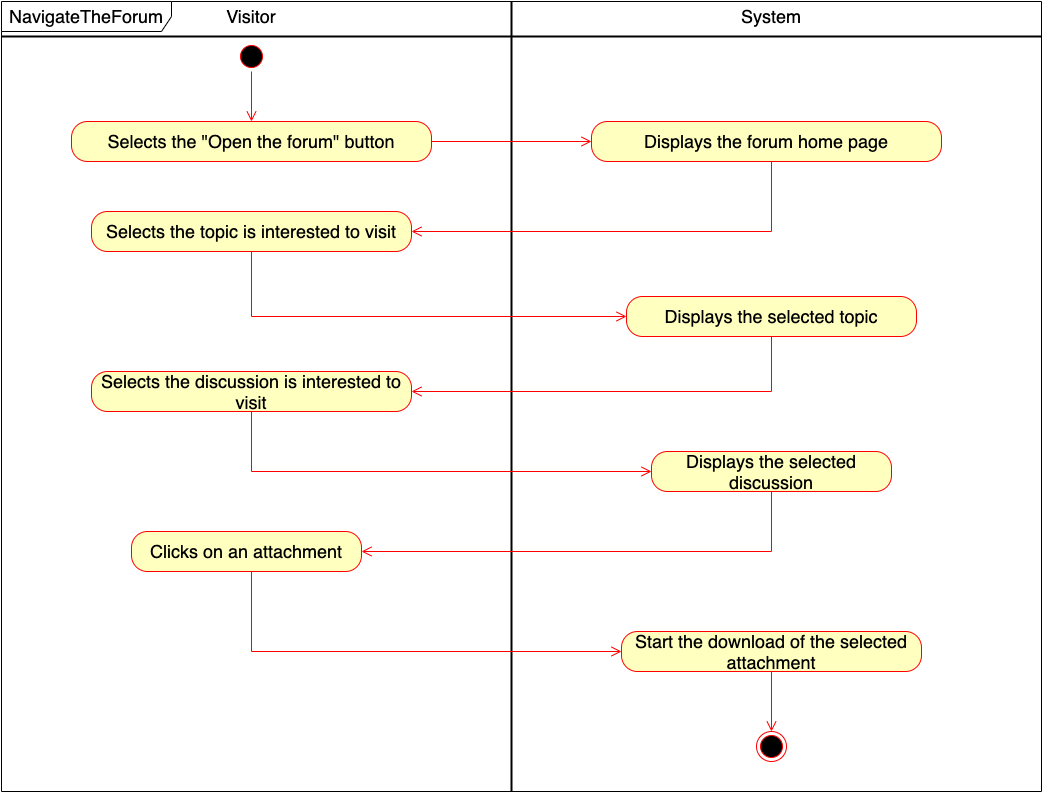
\includegraphics[scale=0.35]{images/use_cases_diagram/visitor_navigate_forum.png}
        \caption{Navigates the forum and download a document}
        \label{fig:navigate_forum}
    \end{figure}
    \FloatBarrier